% ===========================================
% Template for ICMC 2016 (version2)
% adapted from earlier LaTeX paper templates for the ICMC, SMC, etc...
% ===========================================

\documentclass{article}
\usepackage[utf8]{inputenc}
\usepackage{icmc2016template}
\usepackage{times}
\usepackage{ifpdf}
\usepackage{soul}
\usepackage[english]{babel}
\usepackage{listings}
\lstset{columns=fullflexible,keepspaces=true,basicstyle=\ttfamily}
%\usepackage{cite}


%%%%%%%%%%%%%%%%%%%%%%%% Some useful packages %%%%%%%%%%%%%%%%%%%%%%%%%%%%%%%
%%%%%%%%%%%%%%%%%%%%%%%% See related documentation %%%%%%%%%%%%%%%%%%%%%%%%%%
%\usepackage{amsmath} % popular packages from Am. Math. Soc. Please use the 
%\usepackage{amssymb} % related math environments (split, subequation, cases,
%\usepackage{amsfonts}% multline, etc.)
%\usepackage{bm}      % Bold Math package, defines the command \bf{}
%\usepackage{paralist}% extended list environments
%%subfig.sty is the modern replacement for subfigure.sty. However, subfig.sty 
%%requires and automatically loads caption.sty which overrides class handling 
%%of captions. To prevent this problem, preload caption.sty with caption=false 
%\usepackage[caption=false]{caption}
%\usepackage[font=footnotesize]{subfig}

% ====================================================
% ================ Define title and author names here ===============
% ====================================================
%user defined variables
\def\papertitle{Graphical Temporal Structured Programming for Interactive Music}
\def\firstauthor{Anonymized}
\def\secondauthor{Anonymized}
\def\thirdauthor{Anonymized}

%\def\firstauthor{Jean-Michaël Celerier}
%\def\secondauthor{Myriam Desainte-Catherine}
%\def\thirdauthor{Jean-Michel Couturier}

% adds the automatic
% Saves a lot of output space in PDF... after conversion with the distiller
% Delete if you cannot get PS fonts working on your system.

% pdf-tex settings: detect automatically if run by latex or pdflatex
\newif\ifpdf
\ifx\pdfoutput\relax
\else
   \ifcase\pdfoutput
      \pdffalse
   \else
      \pdftrue
  \fi
\fi

\ifpdf % compiling with pdflatex
  \usepackage[pdftex,
    pdftitle={\papertitle},
    pdfauthor={\firstauthor, \secondauthor, \thirdauthor},
    bookmarksnumbered, % use section numbers with bookmarks
    pdfstartview=XYZ % start with zoom=100% instead of full screen; 
                     % especially useful if working with a big screen :-)
   ]{hyperref}
  %\pdfcompresslevel=9

  \usepackage[pdftex]{graphicx}
  % declare the path(s) where your graphic files are and their extensions so 
  %you won't have to specify these with every instance of \includegraphics
  \graphicspath{{./figures/}}
  \DeclareGraphicsExtensions{.pdf,.jpeg,.png}

  \usepackage[figure,table]{hypcap}

\else % compiling with latex
  \usepackage[dvips,
    bookmarksnumbered, % use section numbers with bookmarks
    pdfstartview=XYZ % start with zoom=100% instead of full screen
  ]{hyperref}  % hyperrefs are active in the pdf file after conversion

  \usepackage[dvips]{epsfig,graphicx}
  % declare the path(s) where your graphic files are and their extensions so 
  %you won't have to specify these with every instance of \includegraphics
  \graphicspath{{./figures/}}
  \DeclareGraphicsExtensions{.eps}

  \usepackage[figure,table]{hypcap}
\fi

%setup the hyperref package - make the links black without a surrounding frame
\hypersetup{
    colorlinks,%
    citecolor=black,%
    filecolor=black,%
    linkcolor=black,%
    urlcolor=black
}

\title{\papertitle}

%\threeauthors
%   {0.5in}
%   {\firstauthor} {LaBRI, Blue Yeti \\ %
 %    {\tt \href{mailto:author1@smcnetwork.org}{author1@smcnetwork.org}}}
 %  {\secondauthor} {LaBRI, CNRS \\ %
  %   {\tt \href{mailto:author2@smcnetwork.org}{author2@smcnetwork.org}}}
  % {\thirdauthor} { Blue Yeti \\ %
   %  {\tt \href{mailto:author3@smcnetwork.org}{author3@smcnetwork.org}}}

\begin{document}
%
\capstartfalse
\maketitle
\capstarttrue
%
\begin{abstract}
     The development and authoring of interactive music or applications, such as user interfaces for arts \& exhibitions
     has traditionally been done with tools that pertain to two broad metaphors. 
     Cue-based environments work by making groups of parameters and sending them to remote devices, 
     while more interactive applications are generally written in generic art-oriented 
     programming environments, such as Max/MSP, Processing or OpenFrameworks.
     In this paper, we argue about the specific issues that arise in such environments, and we present 
     the current version of the i-score sequencer. It is an extensive software suite that bridges
     the gap between time-based, logic-based and flow-based interactive application authoring tools. 
     This is done in a single cohesive graphical user interface, built upon a few simple and novel primitives that give to the composer the expressive power of structured programming, in a time line adapted to the notation of parameter-oriented interactive music.    
\end{abstract}
%

\section{Introduction}\label{sec:introduction}
This paper outlines the new capabilities in the current iteration of i-score, 
a free and open-source interactive scoring sequencer.
It is targeted towards the composition of scores that will have 
an interactivity component, that is, that are meant to be performed 
to some extent.
While it can be used for music composition, it is not restricted to solely auditory arts
but can instead control any kind of multi-media work.

We first expose briefely the main ideas behind interactive scores, and explain 
how i-score can now be used as a language of the structured programming language 
family, targeted towards temporal compositions, in a visual time-line interface.

In previous research\cite{hogue2014ossia} interactive triggers were exhibited as a tool for a musician 
to interact with the computer in a compositionnally well-defined way.
Here, we show that with the introduction of loops, and the capacity to perform computations 
on variables in a score, we are able to use interactive triggers as a powerful flow control tool, which 
allows to express event-driven constructs, and to build a notion similar to traditionnal programming 
languages functions.

We conclude by exhibiting an i-score example of a musical work inspired by polyvalent structure music,
that can be used by composers as a starting point. 
This example contains relatively few elements, which shows the practical expresiveness of the language.

\subsection{Temporal multimedia programming}
The sequencer metaphor is common amongst audio engineers : 
tracks, and audio or MIDI clips in these tracks, with applied effects 
and parameter automations that take effect during a period of time.

In multiple cases, it has been shown that it was possible to write 
more generalist multimedia time-line based sequencers, without the need to restrict oneself 
to audio data types. 
The MET++ framework\cite{ackermann1994direct} is an object-oriented framework 
tailored to build such multimedia applications.
A common approach, also used in previous version of i-score, is to use constraint programming 
to represent relations between temporal objects\cite{song1999interactive, allombert2006concurrent, toro2010concurrent}. 
In \cite{hirzalla1995temporal}, Hirzalla shows how conditionality can be introduced in a timeline 
to produce different outcomes for a single time-line.

Other approaches for interactive music are generally not based on the time-line metaphore, 
but more on interaction-centric applications written in patchers such Max/MSP or PureData, 
with an added possibility of scenarisation using cues. 
However, the temporal order is then not apparent from the visual representation of the program, 
unless a lot of care is taken by the composer.

% - références anciens articles i-score 
% - protocoles ?
\section{Syntax}
The syntax and graphical elements used in i-score as well as the 
execution semantics are for the most part introduced in \cite{celerier2015ossia, baltazar2014score}.
Multiple execution semantics for the same graphical formalism have been developed. 
They are based on Petri Nets\cite{allombert2007system}, Time Automata\cite{arias2015exploiting}, reactive languages\cite{arias2014executing} and temporal concurrent constraint programming\cite{toro2010model}.

The novelty lies in the introduction of temporal loops, and of a computation model 
based on Javascript that can be used at any point in the score. 
These two features, when combined, provide more expressive power to the i-score visual language, 
which allows for more dynamic scores.

\subsection{Temporal structured programming}
Structured programming is a programming paradigm which traces 
back to the 1960's, and was conceived at a time where the use of \lstinline{GOTO}
instructions was prevalent in programming, which often led to code difficult to understand.

The structured programming theorem\cite{bohm1966flow,mills1972mathematical} states that any computable function can be computed 
without the use of \lstinline{GOTO} instructions, if instead the following operations are available : 
\begin{itemize}
    \item Sequence (\lstinline{A} followed by \lstinline{B}), 
    \item Conditional (\lstinline{if(Pred) then A else B}), 
    \item Iterative (\lstinline{while(Pred) do A}).
\end{itemize}

Additionnaly, the ability to perform computations is required in order to have a meaningful program.

\begin{figure}
    \centering
    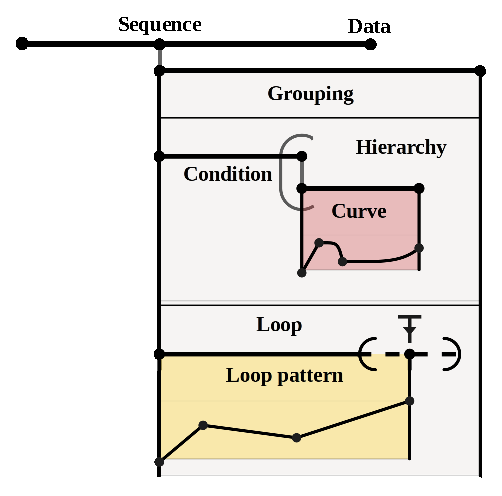
\includegraphics[width=0.40\textwidth]{images/hierarchy.eps}
    \caption{Screenshot of a part of i-score, showing major elements of the formalism. The time constraint is the full or dashed horizontal line, the states are the black dots, the time nodes are the vertical bars, and a time event is shown at the right of the "Condition" text. Interactive triggers are black \textbf{T}'s with a downwards arrow. There are five processes (capitalized) : an englobing Scenario which is the hierarchical root of the score, another Scenario, in the box "Hierarchy", an Automation on a remote parameter in the "Curve" box, a Loop in the box containing the loop pattern, and another Automation that will be looped.}
    \label{fig.hierarchy}
\end{figure}

In order to allow for interactive musical scores authoring, we introduce these concepts in the time-line paradigm.
A virtual machine ticks a timer and makes the time flow in the score graph. 
During this time, multiple processes, including hierarchical scenarisation, looping, and multimedia processes, are 
run at each tick. 

Processes can be of two kinds : temporal or instantaneous.
Temporal processes can be explained as functions of time that the composer wants to run between 
two points in time. 
For instance : \emph{do a volume fade-in from t=10s to t=25s}.~\\
Instantaneous processes are functions that will be run at a single point in time.
For instance : \emph{send a single random number to an OSC address}.

\subsubsection{Scenario}
The scenario is an organisation of the elements of the i-score model : time constraint (a span of time which contains temporal processes), time node (which will synchronize the ending of time constraints with the happening of an external event such as a note being played), time event (a condition that will cause its following time constraints to start if it is true), and state (which contains data to send and instantaneous processes).
They are shown in fig.~\ref{fig.hierarchy}. 
The time flows from left to right as in most traditional sequencers, however due to the presence of interactivity, we cannot show all the possibilities of execution of the score, since they would be almost infinite. 
Hence dashes are shown when the actual execution time is not known beforehand. 
For instance : \emph{play a D minor chord until a dancer moves on stage}.

In the context of a Scenario, these primitives allows for sequencing elements, conditional branching, and interactive triggering, but are not enough for looping.
The GUI of the i-score software allows for all the common and expected operations for elements of a scenario : displacement, scaling, creation, deletion, copy-paste...

\subsubsection{Loop}
The loop is another organization of the same elements, more restrictive, and with a different control flow : it is 
composed exclusively of two time nodes, two time events, two states, and a time constraint in between.
When the second time node gets executed, the time flow is reverted to before the execution of the first time node.
This means that if the composer adds an interactive trigger on any of these time nodes, the Loop will be able to do pattern of different durations at each loop cycle.
This is strictly more general than loops in more traditional sequencers such as Avid Pro Tools, Steinber Cubase or Apple Logic, when the loop is generally a strict duplication of the audio or MIDI data.

\subsubsection{Communication}
The software mainly communicates via the OSC\footnote{Open Sound Control} protocol,  and maintains a tree of parameters able to mirror 
the object model of remote software built with Max/MSP, PureData, Unity3D or any OSC-compliant environment. 
Conditions, interactive triggers, and more generally all processes of i-score have unrestricted 
access to this tree, and can read its data, perform computations on it, and write it back to the 
remote software.
Music can currently expressed with the help of either a remote software or hardware device that is able 
to convert OSC messages to either MIDI or audio.
One can for instance easily build a PureData patch to convert OSC messages matching a certain pattern 
to the corresponding MIDI notes.

\subsection{Variables}
Having variables is important : a variable can hold data, 
and a computation can be performed on it.
For instance : $x \rightarrow x + 1$ is a simple incrementation 
operation, which requires one variable $x$.
Different programming languages have different takes on the 
capabilities of variables.
For instance, functional programming languages will generally 
behave according to immutability rules, that is, a variable once 
assigned cannot be modified.
This is in contrast with imperative languages, closer 
to the machine's memory model with addressable data.

The implementation of variables is based on the device tree, which 
acts like a global memory. 
The composer can create new variables graphically in the tree, and select their types.
While there is no primitive to allow memory allocation during the execution of a score, it could easily be implemented by having a special address that would take in argument the name of the variable to allocate as well as its type.

Finally, there is no notion of scope in the device tree : any process can access to any variable, which 
should be considered elements of the object model of the local software.
However, when local variable are necessary for complex computations, it 
is better to use the embedded scripting language to hide them.
\section{Authoring features}
i-score provides multiple authoring features aiming to allow 
the composer to express himself.
Besides, the software is based on a plug-in architecture which 
allows for easy extension of its capabilities.
\begin{itemize}
\item Javascript support : one can use Javascript scripts both as temporal and instantaneous processes.
When writing a temporal process, the composer has to provide a function of the following form : 
\begin{lstlisting}
function(t) {      
    var obj = new Object; 
    obj.address = '/an/address'; 
    obj.value = 42 * t; 
 return [ obj ]
}
\end{lstlisting}
This function will get called at each tick with the time \lstinline{t} being a floating point between 0 and infinity, 1 being the default date that the composer has set. 
It will produce a linear ramp on the \lstinline|/an/address| parameter, that will go from zero to 42 during the duration of the parent time constraint of this process.
The messages returned will be applied to the local state of the tree and sent remotely if corresponding nodes were found.
When writing an instantaneous process, the function to provide is similar, but does not take a time argument.
Functions writer are encouraged to write stateless functions, since it would allow for optimizations opportunities such as precomputing an array of values.
Finally, a global object provides API functions to query the current state of other parameters in the device tree.
This allows for arbitrarily complex mappings between parameters.

\item Automation : the traditional DAW automation, which writes in a parameter over time. 
Currently provided are 1D (linear, power) and 3D (cubic spline) automations.
\item Mapping : similar in appearance to the automation, this process will take an OSC address as input, apply a transfer function drawn graphically, and write the output to another address.
\item Recording : one can record either automations which will be able to apply automatic interpolation for numeric parameters, or record any kind of input message to replay it afterwards.
\item Execution speed control : the temporal constraints all have a multiplicating coefficient for execution speed.
\item Introspectability : i-score exposes the current score in the same tree that the remote devices. 
Multiple attributes can be queried, and to some extent modified during the execution of the score. 
For instance, the activation status of interactive triggers, and the execution speed of all the temporal constraints are controlable parameters.
The elements are organized hierarchically according to their hierarchy in the scenario, and can also be remote-controled from the network.
Plug-ins can expose their own attributes in this tree.
\item Interactive execution : during the authoring process, it is sometimes necessary to replay just a part of the score.
i-score provides this capacity. 
However, it is necessary for the composer to choose beforehand the truth value of conditions he wants to test.
There are two "debug" execution modes : one that will directly start playing from where the user points the mouse, and another that will try to merge all the previously sent values, to put the external environment in the same state that it would be if the score had been played normally up until this point. 
This breaks if there are physical processes that are not instantaneous, as would be the case for smoke machines for instance.
\end{itemize}
\section{Temporal design patterns}
In this section, we present various design patterns that can be used 
when one wants to build an interactive score with i-score.
We will showcase event-driven scores, which will have a behaviour 
similar to a traditional computer program executing instruction after 
instruction at maximal speed, and an example in simulating the 
concept of function in a time-driven model.
\subsection{Event-driven design}
\begin{figure}
    \centering
    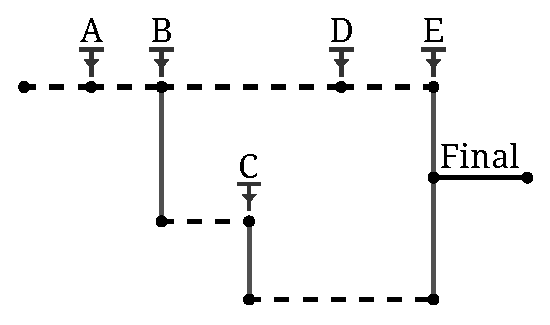
\includegraphics[width=0.45\textwidth]{images/event.eps}
    \caption{An example of event-driven score}
    \label{fig.event}
\end{figure}
Event-driven, or asynchronous design is a software design 
paradigm that is centered on the notion of asynchronous 
communication between different parts of the software.
This is commonly used when doing networked operations or 
user interfaces, since they have to be responsive.

One would write, in a (poor) imperative style : 
\begin{lstlisting}
play A
wait for the end of A
play B
wait for the end of B
play C
\end{lstlisting}
In event-driven programming, instead, one would write a software 
using callbacks, futures or reactive programming patterns\cite{kambona2013evaluation} :~\\
\begin{lstlisting}
when A is triggered
    play B
when B is triggered
    play C    
play A
\end{lstlisting}

Since i-score supports interactive events, one can easily write such event chaining.
An example is given in fig.~\ref{fig.event}. 
The advantage is that ordered operations can be written easily : there is no 
possibility for B to happen before A if there is a time constraint between A and B.
However, the execution engine will introduce a delay of one tick between each call.
The tick frequency can be set to as high as one kilo-hertz.
Synchronization can also be graphically explicited : here, the last time constraint, in solid black, will 
only be executed after all the incoming branches were executed. 
This allow to write a score that says : \emph{start section B five seconds after musician 1 and 3 
have stopped playing}.
There is no practical limit to the amount of branches that can be synchronized in this way.

\subsection{Simulating functions}

\begin{figure}
\centering
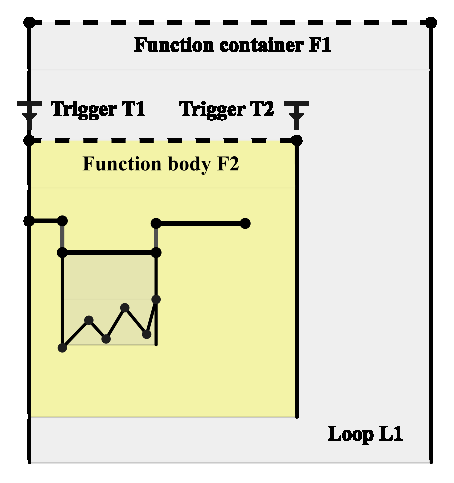
\includegraphics[width=0.40\textwidth]{images/function.eps}
\caption{Implementation of a function in i-score}
\label{fig.function}
\end{figure}

The notion of function is extremely common in programming languages.
It consists in an abstraction around a behaviour that can be called 
by name easily.
The concept of function is useful, because it means that 
if one wants the same behaviour to occur at multiple times during
the execution of the program or the score, this behaviour will 
have to be written only once.
However, the visual flow becomes destructured, because 
the definition of the function is given at a point in the program / score, 
and its usage is at other points.

We present in fig.~\ref{fig.function} how one could create a simple 
notion of function that will then be able to be recalled at any point in time.
However, it suffers from a restriction due to its temporal nature : 
it will only be able to be called when it is not already currently running. 
This is due to the single-threaded nature of the execution engine : there is 
only a single "playhead" for the entirety of the score, hence it cannot play the 
same data at two different times.

The function is built as follows : 
\begin{itemize}
    \item A time constraint in the root Scenario will end on an interactive triggering set with infinite duration.
    \item This time constraint contains a Loop process. 
    The functions is named \lstinline{f} in the local tree. The interactive triggers $T_1, T_2$ at the beginning and end of the pattern time constraint are set as follows : 
    \begin{itemize}
        \item $T_1$ : \lstinline{/f/call true}.
        \item $T_2$ : \lstinline{/f/call true}.
    \end{itemize}
    A state triggered by $T_1$ should set the message:~\\
    \lstinline{/f/call false}. This is so that the function does not loop 
    indefinitely and has to be triggered manually again.
    \item The loop contains the actual "function", that is, the process that the composer wants to be able to call from any point in his score. 
\end{itemize}

The execution of this process will then overlay itself with what is currently playing when at another point of the score, 
the message \lstinline{/f/call true} is sent.
Once the function's execution is finished, it enters a waiting state until it is called again.
This behaviour is adapted to interactive arts : generally, one will want to start multiple 
concurrent processes (one to manage the sound, one to manage videos, one to manage lights\dots) at a single point in time; this method allows to implement this.

\section{Musical example : polyvalent structure}
\begin{figure}
    \centering
    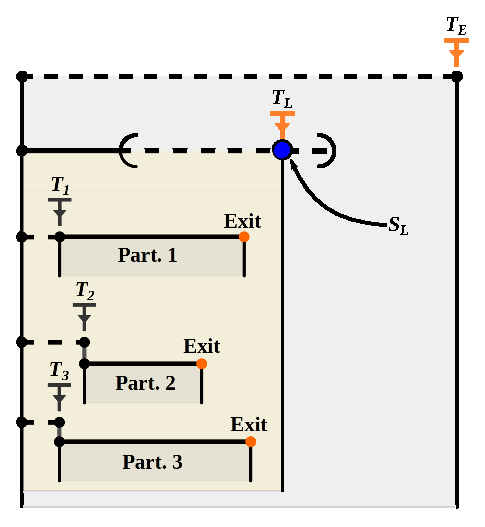
\includegraphics[width=0.45\textwidth]{images/partition.eps}
    \caption{A polyvalent score in i-score}
    \label{fig.polyvalent}
\end{figure}

In this example, showcased in fig.~\ref{fig.polyvalent}, we present a work that is similar in structure to Karlheinz Stockhausen's \emph{Klavierstück XI} (1956), or John Cage's \emph{Two} (1987). 

The complete work contains variables in the tree, as explained earlier, and a temporal score.

The tree is defined as follows : 
\begin{lstlisting}
/part/next    [int = 0]
/part/1/count [int = 0]
/part/2/count [int = 0]
/part/3/count [int = 0]
/exit         [bool = false]
\end{lstlisting}
For instance, \lstinline{/part/next} is an address of integral type, with a default value of zero. 
The score is as follows : there are multiple muscial parts containing recordings of MIDI notes : \textbf{Part. 1, 2, 3}.
These parts are contained in a Scenario, itself contained in a Loop that will run indefinitely. 
At the end of each part, there is an orange State that will write a message "true" to a variable \lstinline{/exit}.
The time constraint of the loop ends on an orange interactive trigger, $T_{loop}$.
The Loop itself is inside a Time constraint ended by an interactive trigger, $T_{end}$.
Finally, the parts are started by interactive triggers  $T_{\{1, 2, 3\}}$ .

The conditions in the triggers are as follows : 
\begin{itemize}
\item  $T_{\{1, 2, 3\}}$ : \lstinline|/part/next == {1, 2, 3}|.
\item $T_{loop}$ : \lstinline{/exit == true}.
\item $T_{end}$ : ~\\
\lstinline{/part/1/count > 2 or} \\
\lstinline{/part/2/count > 2 or} \\
\lstinline{/part/3/count > 2}.
\end{itemize}

Finally, the pink state under $T_{loop}$ contains a Javascript function 
that will draw a random number between 1 and 3, 
increment the count of the relevant \verb|/part|, 
and write the drawn part in \verb|/part/next|.
If any count becomes greater than two, then $T_{end}$
trigger will stop the execution : the score has ended. 
Else a new loop iteration is started, and either 
$T_1$, $T_2$ or $T_3$ will start instantaneously.

Hence we show how a somewhat complex score logic 
can be implemented with few syntax elements.

Another alternative, instead of putting MIDI data in the score,
which makes it entirely automatic,  
would be to control a screen that displays the part that is 
to be played.
A pianist would then have to interpret the part 
in real-time which would bring back the human aspect.

\section{Tooling}
There are plenty of parts that requires new problems to be solved in i-score, especially in the area of debugging. 
For instance, debugging is generally used to understand and find out easily why did not a program produce the expected result.
In i-score, there is no low-level memory management which removes a large class of errors.
However, as soon as the song's logic becomes complex, it is useful to have tools that give the authors the possibility to pinpoint where the execution of the show does not match the expected behaviour.
Since the presented formalism has extensive expressive capabilities, the composer might find himself confronted to the same family of problems that programmers encounter daily.
Nowadays, many programming language offer very robust tooling, as can be seen in the performance tools that are provided in integrated development environments such as Xcode, Visual Studio, and the various Unix development tools ecosystem\cite{spinellis2014software}.
Such tooling can decrease the development time a lot, and we argue that it would also lead composers to write interactive scores more efficiently.

\section{Conclusion}
We presented ...

We aim to ...

Drawbacks...
% \begin{itemize}
% \item plug-in architecture
% \item open-source
% \item soon : audio and midi support (midi can be done today with osc wrappers but a piano-roll or sheet music view would be nice)
% \item computation graph may be useful to plug the input of a box  to an output without using the tree
% \item other features : spatial, etc.
% \item embeddable 
% \item problématique de déboguage, analyse statique
% \end{itemize}
% - dire qu'on veut utiliser des retours sur les utilisations  les plus courante de JS par les gens pour en faire des éléments  prédéfinis de l'interface graphique.
\begin{acknowledgments}
    Anonymized %This work is supported by an ANRT CIFRE convention with the company Blue Yeti under funding 1181-2014.    
\end{acknowledgments} 

\bibliography{icmc2016template}

\end{document}
